\chapter{Haskell to First Order Logic}

To enable automated theorem provers to do equational reasoning of
Haskell programs a translation to first order logic is needed. It is
here referred to as a translation, but it could also be regarded as a
compilation. The idea is to use constants and functions in first order
logic to correspond to constructors and functions, and arguments to
functions need to be universally quantified. We shall try to do a
na\"{\i}ve attempt of a translation with this ideas and see how far it
takes us.

\section{Na\"{\i}ve Translation}

We will use a data type of binary trees with an element at every
branch, and consider some examples of functions defined on it. This
is the Haskell definition of the data type we will be using:

\begin{code}
data Tree a = Fork (Tree a) a (Tree a) | Leaf
\end{code}

\noindent
With the idea above, occurrences of the \hs{Fork} constructor in the
source code should be translated to a logic function $\fn{fork}$, and
similarly a constant for \hs{Leaf}. How should we then translate the
\hs{singleton} function, defined below?

\begin{code}
singleton :: a -> Tree a
singleton x = Fork Leaf x Leaf
\end{code}

\noindent
Following our intuition we make an universal quantification for
\hs{x}, and a new logic function for \hs{singleton}. The result
is this axiom:
\begin{equation*}
\fa{x} \fn{singleton}(x) = \fn{fork}(\fn{leaf},x,\fn{leaf})
\end{equation*}

\noindent
So far so good, but what if someone wants to prove that \hs{singleton x}
is a \hs{Leaf}? With only this axiom in the theory, it would be
possible: there are models with only one element where \hs{Leaf} is
equal to \hs{Fork}. Indeed, we will need to add axioms that values
created from the different constructors are unequal. We will call
those disjoint constructor axioms, and for the \hs{Tree} data type, we
get this axiom:
\begin{equation*}
\faaa{l}{x}{r} \fn{leaf} \neq \fn{fork}(l,x,r)
\end{equation*}

Constructors should also be injective to get regular models, and
adding such axioms are straightforward. Since only \hs{Fork} has
arguments, this injectivity axiom is needed:
\begin{equation*}
\faaaaaa{l_0}{l_1}{x_0}{x_1}{r_0}{r_1} \fn{fork}(l_0,x_0,r_0) \eq
\fn{fork}(l_1,x_1,r_1) \rightarrow l_0 \eq l_1 \wedge x_0 \eq x_1 \wedge r_0 \eq r_1
\end{equation*}

For the \hs{mirror} function, which recursively mirrors the left sub
tree with the right and vice-versa, we follow our intuition to
translate the pattern matching and get these two axioms\footnote
{Axioms are enumerated by Roman numerals to tell them apart.}:

\begin{code}
mirror :: Tree a -> Tree a
mirror (Fork l x r) = Fork (mirror r) x (mirror l)
mirror Leaf         = Leaf
\end{code}
\begin{align*}
\rom{1} && \faaa{l}{x}{r} & \fn{mirror}(\fn{fork}(l,x,r)) \eq \fn{fork}(\fn{mirror}(r),x,\fn{mirror}(l)) \\
\rom{2} &&                & \fn{mirror}(\fn{leaf}) \eq \fn{leaf}
\end{align*}

\noindent
A problem with this translation is that there are no axioms for other
arguments of $\fn{mirror}$ than leafs and forks, and we have models that
include other values than leafs and forks. Another problem is
encountered for \hs{singleton}'s left inverse, \hs{top}, code below,
which returns the top element of a \hs{Tree}. This is a partial
function since it has no pattern for the \hs{Leaf} constructor.

\begin{code}
top :: Tree a -> a
top (Fork l x r) = x
\end{code}

The translation must capture the pattern match failure that results
from trying to evaluate top applied to a leaf. We conclude that
this na\"{\i}ve translation does not take us further, but we shall see
in the next section how to fix this.

\section{Bottom and Pattern Matching}

In domain theory there is a concept of bottom, denoted $\bot$. It is
used for the least defined value: pattern match failures, use of
\hs{error} and \hs{undefined} in the source code, but also for
non-terminating programs. For \hs{top} the idea is to add an axiom so
that $\fn{top}$ of anything that is not a \hs{Fork} is bottom. This is
an example of such an axiomatization:

\begin{align*}
\rom{1} \qquad & \faaa{l}{x}{r} \fn{top}(\fn{fork}(l,x,r)) \eq x \\
\rom{2} \qquad & \fa{t}         (\nexxx{l}{x}{r} \fn{fork}(l,x,r)) \eq t) \rightarrow \fn{top}(t) \eq \bot
\end{align*}

Most theorem provers would as a preprocessing step \note{\qquad \qquad citation
  needed}skolemize the existential quantification in the second
axiom. A new unary function would be introduced for $l$, $x$ and $r$,
depending on $t$, an arbitrary choice of names are $\fn{top}$ appended
to the original variable. The axiom then looks like
this\footnote{Lambda functions bind as far to the right as possible,
  and this thesis uses the same convention for quantifiers.}:
\begin{align*}
\rom{2}' \qquad & \fa{t} \fn{fork}(\fn{topl}(t),\fn{topx}(t),\fn{topr}(t))) \neq t \rightarrow \fn{top}(t) \eq \bot
\end{align*}

For another function, like \hs{mirror} above, one of the skolemized
functions could be called $\fn{mirrorl}$. Since axioms of injective
constructors are also added, a theorem prover could, in some steps,
conclude that $\faaa{l}{x}{r} \fn{mirrorl}(\fn{fork}(l,x,r)) \eq
\fn{topl}(\fn{fork}(l,x,r)) \eq l$. But what happens if we introduce
such skolemized ``selector'' functions for every constructor manually?
For the \hs{Fork} constructor call them $\fn{fork_0}$, $\fn{fork_1}$
and $\fn{fork_2}$, and their axioms are:
\begin{align*}
\rom{1} \qquad \faaa{l}{x}{r} \fn{fork_{0}}(\fn{fork}(l,x,r)) & \eq l \\
\rom{2} \qquad \faaa{l}{x}{r} \fn{fork_{1}}(\fn{fork}(l,x,r)) & \eq x \\
\rom{3} \qquad \faaa{l}{x}{r} \fn{fork_{2}}(\fn{fork}(l,x,r)) & \eq r
\end{align*}

\noindent
The translation of \hs{top} with these selector functions is:
\begin{align*}
\rom{1} \qquad & \faaa{l}{x}{r} \fn{top}(\fn{fork}(l,x,r)) \eq x \\
\rom{2} \qquad & \fa{t}         (\fn{fork}(\fn{fork_0}(t),\fn{fork_1}(t),\fn{fork_2}(t))) \neq t) \rightarrow \fn{top}(t) \eq \bot
\end{align*}

\noindent
Another nice side effect of writing in this skolemized selector style
is that implies injective constructors. Assume we have
$\fn{fork}(l_0,x_0,r_0)=\fn{fork}(l_1,x_1,r_1)$ then the first
projection, $\fn{fork_0}$, gives us that $l_0=l_1$. Analogously, and
the second and the third give $x_0=x_1$ and $r_0=r_1$,
respectively. Thus selector axioms are added in place of of
injectivity axioms.

With the bottom constant in the theory, the axioms disjointedness are
effected by this. It can be seen as an implicit constructor for every
data type. For the \hs{Tree} data type the axioms are:

\begin{align*}
\rom{1} \qquad & \faaa{l}{x}{r} \fn{fork}(l,x,r) \neq \fn{leaf} \\
\rom{2} \qquad & \faaa{l}{x}{r} \fn{fork}(l,x,r) \neq \bot      \\
\rom{3} \qquad & \bot \neq \fn{leaf}
\end{align*}

Now we have a good idea how to translate pattern matching, but
in Haskell we can pattern match almost everywhere! How would we
proceed to translate a function like this, taken from the
implementation of \hs{scanr} from the \hs{Prelude}?

\begin{code}
scanr             :: (a -> b -> b) -> b -> [a] -> [b]
scanr f q0 []     =  [q0]
scanr f q0 (x:xs) =  f x q : qs
                     where qs = scanr f q0 xs
                           q = case qs of
                                 q : _ -> q
\end{code}

\noindent
There is both pattern matching on the direct arguments, but also
pattern matching in a case statements in the where function
\hs{q}. There can also be pattern matching in lambdas. To help with
these difficulties, we define an intermediate language in the next
section.

\section{The Intermediate Language}

To address the difficulties of pattern matching elsewhere than the
arguments of a function, a small intermediate language was designed
that can only do pattern matching at a very controlled location: in a
case statement that is the entire body of a function, and all arms are
just simple expressions consisting of function and constructor
applications and variables. Haskell is translated to this, and pattern
matching at other locations is translated to this in a new top level
definition. Functions definined in let and where are raised to the top
level, with the necessary variables in scope as additional
arguments. The same is done for sections and lambda functions. The BNF
for the language is this:

\begin{equation*}
\begin{aligned}
\text{Variables} \quad & x \\
\text{Functions} \quad & f \\
\text{Constructors} \quad & C \\
\text{Type variables} \quad & \tau \\
\text{Type constructors} \quad & T \\
\defBNF{Declarations}{decl}{ f \; \overline{x} \; \hs{=} \; body}{function declaration} \\
    \defaltBNF{f \; :: \; t}{type signature} \\
    \defaltBNF{\hs{data} \; T \; \overline{\tau} \; \hs{=} \; \overline{C \; \overline{t}}}{data type declaration} \\
\defBNF{Function body}{body}{\hs{case} \; e \; \hs{of} \; \overline{alt}}{case body} \\
    \defaltBNF{e}{expression body} \\
\defBNF{Expressions}{e}{x}{variable} \\
    \defaltBNF{f \; \overline{e}}{function application} \\
    \defaltBNF{C \; \overline{e}}{constructor application} \\
\defBNF{Alternative}{alt}{pat \rightarrow e}{branch without guard} \\
    \defaltBNF{pat \; \hs{|} \; e \rightarrow e}{branch with guard} \\
\defBNF{Pattern}{p}{x}{pattern variable} \\
    \defaltBNF{C \; \overline{p}}{constructor pattern} \\
\defBNF{Types}{t}{\tau}{type variable} \\
    \defaltBNF{t \; \rightarrow \; t}{function type} \\
    \defaltBNF{T \; \overline{\tau}}{type constructor application} \\
\defBNF{Programs}{prog}{\overline{decl}}{} \\
\end{aligned}
\end{equation*}

This language is a strict subset of Haskell. Repeated entities are
notated with an $\overline{\text{overline}}$.  Data declarations are
added for disjointedness and selector axioms, and type signatures are
just skipped in the translation, but the proof techniques introduced
later use this information.

A function is just a function name with a number of variables, and
then a function body, which is either an expression of variables,
functions and constructors, or a case statements with an expression
scrutinee. Branches consists of a pattern, possibly with nested uses
of constructors, and an optional guard, and in the arm is an
expression.

Now we need to distinguish between two translations: the intermediate
translation from Haskell to the intermediate language, and the logic
translation from this language to first order logic.

\section{The Intermediate Translation}

After this section, we will only concentrate on the logic translation.

\paragraph{Argument pattern matching} A function that does pattern matching will be translated to one that
takes in unmatched arguments and with a case in the body. The
\hs{mirror} function above is thus translated to this:

\begin{code}
mirror :: Tree a -> Tree a
mirror t = case t of
   Fork l x r -> Fork (mirror r) x (mirror l)
   Leaf       -> Leaf
\end{code}

\noindent
If you do pattern matching on several arguments, the scrutinee in the
case will be a tuple of all the arguments.

\paragraph{Local definitions} Where-clauses and let-expressions are
raised to the top level, with all necessary variables as
arguments. This example of an accumulator definition of multiplication
of Peano natural numbers needs such a rewrite:

\begin{code}
(*) :: Nat -> Nat -> Nat
x * y = go Zero x
  where
    go acc Zero    = acc
    go acc (Suc n) = go (acc + y) n
\end{code}

\noindent
The \hs{go} function has the \hs{y} in scope but not as argument so it
is appended to the arguments to the top level lifted version of \hs{go}:

\begin{code}
go acc Zero    y = acc
go acc (Suc n) y = go (acc + y) n y

x * y = go Zero x y
\end{code}

\noindent
Finally \hs{go} is translated using a case expression:

\begin{code}
go acc x y = case x of
     Zero  -> acc
     Suc n -> go (acc + y) n y
\end{code}

A similar translation is done for let expressions.

\paragraph{Lambda functions} These are translated to top level
definitions. Take this example of defining \hs{fmap} in terms of the
functions from the \hs{Monad} type class:

\begin{code}
fmap' :: Monad m => (a -> b) -> m a -> m b
fmap' f m = m >>= \x -> return (f x)
\end{code}

\noindent
In the lambda, \hs{f} is a free variable so it becomes an argument to
the new top level function called \hs{lambda} below:

\begin{code}
lambda f x = return (f x)

fmap' :: Monad m => (a -> b) -> m a -> m b
fmap' f m = m >>= lambda f
\end{code}

A similar translation is done for sections.

\section{Pattern Matching Revisited}

\paragraph{Overlapping patterns} First of all, overlapping patterns need to be removed, otherwise we
easily get an inconsistent theory, consider

\begin{code}
overlap :: Bool -> Bool
overlap b = case b of
              True -> True
              True -> False
\end{code}

Certainly, this cannot be translated to:
\begin{align*}
\rom{1} \qquad & \fn{overlap}(\fn{true}) = \fn{true} \\
\rom{2} \qquad & \fn{overlap}(\fn{true}) = \fn{false} \\
\rom{3} \qquad & \fa{b} b \neq \fn{true} \rightarrow \fn{overlap}(b) = \bot
\end{align*}

Starting from the immediate truth $\fn{overlap}(\fn{true}) =
\fn{overlap}(\fn{true})$, transitivity of the equalities in the axioms
$\romnodot{1}$ and $\romnodot{2}$ gives the equality $\fn{true} =
\fn{false}$. This together with the axiom from disjoint constructors,
$\fn{true} \neq \fn{false}$, gives a contradiction.

In Haskell, pattern matching is done from top to bottom of the
definition, making the second match of \hs{True} to never occur. Thus,
the translation to FOL also removes all subsequent patterns that are
instances of any pattern above.

\paragraph{Nested patterns and bottoms} The translation also handles
patterns in more than one depth. At every location in a pattern where
a constructor is matched against, a pattern with bottom at that spot
is also added, defined to bottom. This Haskell function \hs{even}
determines if a list is of even length:

\begin{code}
even :: List a -> Bool
even (Cons x (Cons y ys)) = even ys
even (Cons x xs)          = False
even Nil                  = True
\end{code}

\noindent
For the sake of readability it is not presented with a case
expression, though this is what the intermediate translation would
transform it to. Furthermore the constructors \hs{Cons} and \hs{Nil}
are used since the projections $\fn{:_0}$ and $\fn{:_1}$ for the
normal cons are hard to read.

For each matched constructor, we need to add a new match to bottom,
which evaluates to bottom. Unnecessary bottoms can be carelessly added
since overlapping patterns are removed \emph{afterwards}. Furthermore,
a wild pattern is added at the end that goes to bottom in case there
are other constructors for the data type not mentioned in the
patterns.

No type information is needed to do this: it is merely an
inspection. Could the bottoms be seen in this Haskell definition it
would be this after the insertion of bottoms:

\begin{code}[mathescape]
even :: List a -> Bool
even (Cons x (Cons y ys)) = even ys
even (Cons x $\bot$)            = $\bot$
even $\bot$                     = $\bot$
even (Cons x xs)          = False
even Nil                  = True
even _                    = $\bot$
\end{code}

Haskell's behavior of matching patterns from top to bottom is
justified with implications ensuring the \emph{upward agreement}. The
axioms for this definitions are:
\newcommand\uncons[1]{\cons{\fn{cons_0}(#1)}{\fn{cons_1}(#1)}}
\newcommand\even[1]{\fn{even}(#1)}
\newcommand\cons[2]{\fn{cons}(#1,#2)}
\begin{align*}
\rom{1} && \faaa{x}{y}{ys} & \even{\cons{x}{\cons{y}{ys}}} = \even{ys} \\
\rom{2} && \fa{x}          & \even{\cons{x}{\bot}}         = \bot      \\
\rom{3} &&                 & \even{\bot} = \bot \\
\rom{4} && \faa{x}{xs}     & xs \neq \uncons{xs} \wedge xs \neq \bot \rightarrow \even{\cons{x}{xs}} = \fn{false}  \\
\rom{5} &&                 & \even{\fn{nil}} = \fn{true} \\
\rom{6} && \fa{xs}         & xs \neq \fn{nil} \wedge
                             xs \neq \uncons{xs} \wedge
                             xs \neq \bot \rightarrow \even{xs} = \bot
\end{align*}

Some room for improvement can be seen: the inserted
\hs{even }$\bot$\hs{ = }$\bot$ case is redundant as it is implied by
the wild pattern to $\bot$. The upward agreement implications can
readily be seen, an example is
$xs \neq \uncons{xs} \wedge xs \neq \bot$ in axiom $\romnodot{3}$.

\section{Functions as Arguments}

In Haskell, functions readily take other functions as arguments, and
functions can also be partially applied. To get the same behavior in
logic, each function gets a \emph{function pointer}, and a new binary
function is added to the language, written infix with $\appfn$.  For
instance if there is a binary function \hs{plus} then a constant
called $\fn{plus.ptr}$ is added to the theory and this axiom:

\begin{equation*}
\faa{x}{y}  \app{(\app{\fn{plus.ptr}}{x})}{y} = \fn{plus}(x,y)
\end{equation*}

When a function is only partially applied, or a function argument is
applied, $\appfn$ is used. Consider this Prelude function \hs{iterate}:

\begin{code}
iterate :: (a -> a) -> a -> [a]
iterate f x = x : iterate f (f x)
\end{code}

It is translated with $\appfn$ in the following way, with the cons
constructor \hs{:} written infix:

\begin{equation*}
\forall \, f \, x \, . \, \fn{iterate}(f,x) = x : \fn{iterate}(f,\app{f}{x})
\end{equation*}

Should a function not get all its arguments, appropriate use of $\, @ \, $ is
added, as in this function which increments all elements of the list
by one using \hs{map}:

\begin{code}
incr = map (plus one)
\end{code}

As \hs{incr} is written $\eta$-reduced, \hs{map} is
only partially applied, this is the translated axiom:

\begin{equation*}
\fn{incr} = \app{\fn{map.ptr}}{(\app{\fn{plus.ptr}}{\fn{one}})}
\end{equation*}

If \hs{incr} is applied to an argument $xs$, then \hs{incr} is applied
to more arguments than it takes, so we add $\appfn$ so the
corresponding formula becomes $\app{\fn{incr}}{xs}$, and by equational
substitution from the definition of $\fn{incr}$ we get
$\app{(\app{\fn{map.ptr}}{(\app{\fn{plus.ptr}}{\fn{one}})})}{xs}$ and
the axiom of $\fn{map.ptr}$ then equals this to
$\fn{map}(\app{\fn{plus.ptr}}{\fn{one}},xs)$.

\section{Guards}

Guards are treated much like pattern matching. If a
guard expression evaluates to \hs{True}, that branch is picked. The
expression could also evaluate to $\bot$, and then the result should
be $\bot$. Let us consider the \hs{filter} function:

\begin{code}
filter :: (a -> Bool) -> List a -> List a
filter p (Cons x xs) | p x = Cons x (filter p xs)
filter p (Cons x xs)       = filter p xs
filter p Nil               = Nil
\end{code}


To translation this to logic it is needed to ensure that if \hs{p x}
evaluates to $\bot$, then so should the function. The axioms look
like this:
\newcommand\filter[2]{\fn{filter}(#1,#2)}
\begin{align*}
\rom{1} && \faaa{p}{x}{xs} & (\app{p}{x}) = \fn{true}                                  \rightarrow \filter{p}{\cons{x}{\cons{y}{ys}}} = \cons{x}{\filter{p}{xs}} \\
\rom{2} && \faaa{p}{x}{xs} & (\app{p}{x}) = \bot                                       \rightarrow \filter{p}{\cons{x}{\cons{y}{ys}}} = \bot \\
\rom{3} && \faaa{p}{x}{xs} & (\app{p}{x}) \neq \fn{true} \wedge (\app{p}{x}) \neq \bot \rightarrow \filter{p}{\cons{x}{\cons{y}{ys}}} = \filter{p}{xs} \\
\rom{4} &&                 & \filter{p}{\fn{nil}} = \fn{nil} \\
\rom{5} && \fa{xs}         & xs \neq \fn{nil} \wedge xs \neq \uncons{xs} \rightarrow \filter{p}{xs} = \bot
\end{align*}

\section{Summary}

The translation of different Haskell concepts is summarized in
Table~\ref{tab:transtable}.

\begin{table}[h]
  \centering
  \begin{tabular}{|l|l|}
    \hline
    Haskell                    & First Order Logic \\
    \hline
    function                   & function or constant \\
    constructor                & function or constant \\
    data type                  & disjoint constructors and selector axioms \\
    pattern matching           & overlap removal, bottoms insertion, upward agreement \\
    guards                     & equality to true and bottom and upward agreement \\
    partial application        & $\appfn$ on pointer constant \\
    partially applied function & pointer constant and $\appfn$ rule \\
    sections, lambdas, let     & new functions with variables in scope as arguments \\
    \hline
  \end{tabular}
  \caption{Translation of different Haskell constructs
    \label{tab:transtable}
  }
\end{table}

%Equational reasaoning is traditional in proving corrected of Haskell
%programs, but it assumes that a simple denotational semantics exists,
%and there is not even a formal semantics for the language
%\cite{chasingbot}.
%

% Remove unnecessary definitions for a given proof


%% Domain theory

\section{Domain Theory}
\label{sec:domaintheory}

This section is stand alone, and could be skipped especially if you
already know the basics of Domain Theory: comp\-lete partial orders,
monotonicity and continuity.
It explains these concepts and discusses how it can be
used to verify the translation, furthermore it is used as a reference
in the future sections that rely on concepts from domain theory.
%The section explains these concepts and acts as a reference in future
%sections that rely on concepts from domain theory.

The values of every data type are ordered on how much ``information''
they contain. The least element bottom, denoted $\bot$, contains least
information. It corresponds to all kinds of crashes in Haskell; use of
\hs{undefined}, non-termination or non exhausite pattern matches.
Different constructors hold different information, so they are not
related by the ordering; this is a partial order, a relation that is
reflexive, transitive and antisymmetric. The ordering is usually
written $\sqsubseteq$ sometimes with a subscript indicating the type.

\begin{wrapfigure}{O}{0.4\textwidth} %\begin{figure}
\vspace{-7pt}
\centering \begin{tikzpicture}[
    level distance=-1.5cm,
    growth parent anchor=north,
    sibling distance=3cm
]
\node {$\bot$}
    child {
        node {$\hs{True}$}
    }
    child {
        node {$\hs{False}$}
    };
\end{tikzpicture}


%\end{document}
\vspace{-7pt}
\caption{
    The order of Bool values.
    \label{fig:boolcpo}
}
\end{wrapfigure}
For the \hs{Bool} data type the partial order can be drawn as a Hasse
Diagram and this can be shown in Figure \ref{fig:boolcpo}.  From the
picture it is understood that $\bot$ is the least element, and the
line from it to \hs{False} means that $\bot \sqsubseteq \hs{False}$,
since $\bot$ is below $\hs{False}$. Correspondingly for $\hs{True}$,
the diagram tells us that $\bot \sqsubseteq \hs{True}$. It can also
been seen that $\hs{True} \nsqsubseteq \hs{False}$; they are unrelated
since there is no line between them.

%\begin{figure}[h]
%\centering
%\begin{tikzpicture}[
    level distance=-1.5cm,
    growth parent anchor=north,
    sibling distance=3cm
]
\node {$\bot$}
    child {
        node {$\hs{True}$}
    }
    child {
        node {$\hs{False}$}
    };
\end{tikzpicture}


%\end{document}
%\caption{The partial order for \texttt{Bool} as a Hasse Diagram
%  \label{fig:boolcpo}
%}
%\end{figure}

%\begin{figure}[h]
%  \centering
%  \subfloat[\texttt{Bool}]{\label{fig:boolcpo}\begin{tikzpicture}[
    level distance=-1.5cm,
    growth parent anchor=north,
    sibling distance=3cm
]
\node {$\bot$}
    child {
        node {$\hs{True}$}
    }
    child {
        node {$\hs{False}$}
    };
\end{tikzpicture}


%\end{document}}
%  \hspace{20pt}
%  \subfloat[\texttt{(Bool,Bool)}]{\label{fig:boolboolcpo}%\documentclass[10pt]{article}
\newcommand{\myGlobalTransformation}[2]
{
    \pgftransformreset;
    \pgftransformcm{1.6}{0}{0.6}{0.5}{\pgfpoint{#1cm}{#2cm}}
}

\newcommand\tru{\hs{T}}
\newcommand\fal{\hs{F}}

\newcommand\ddraw[2]{
        \draw[-,line width=3pt,draw=white] (#1) -- (#2);
        \draw (#1) -- (#2);
}

%\begin{document}
%\pagestyle{empty}

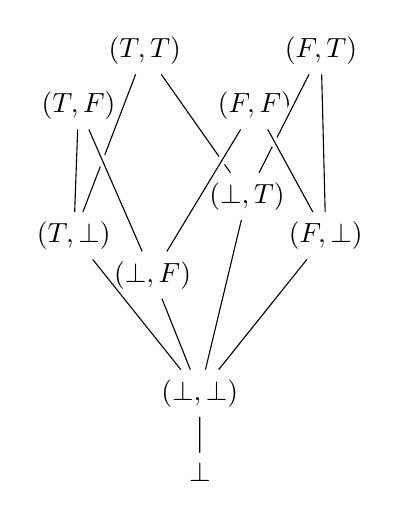
\begin{tikzpicture}

    \begin{scope}
        \myGlobalTransformation{0}{0};
        \node (bottom) at (0,0) {$\bot$};

        \myGlobalTransformation{0}{1};
        \node (botbot) at (0,0) {$(\bot,\bot)$};

        \myGlobalTransformation{0}{3};
        \node (trubot) at (-1,0) {$(\tru,\bot)$};
        \node (bottru) at (0,1)  {$(\bot,\tru)$};
        \node (falbot) at (1,0)  {$(\fal,\bot)$};
        \node (botfal) at (0,-1) {$(\bot,\fal)$};

        \myGlobalTransformation{0}{5};
        \node (trutru) at (-0.7, 0.7) {$(\tru,\tru)$};
        \node (faltru) at ( 0.7, 0.7) {$(\fal,\tru)$};
        \node (falfal) at ( 0.7,-0.7) {$(\fal,\fal)$};
        \node (trufal) at (-0.7,-0.7) {$(\tru,\fal)$};

        \draw (bottom) -- (botbot);

        \draw (botbot) -- (trubot);
        \draw (botbot) -- (bottru);
        \draw (botbot) -- (falbot);
        \draw (botbot) -- (botfal);

        \ddraw{trubot}{trutru};
        \ddraw{bottru}{trutru};
        \ddraw{falbot}{faltru};
        \ddraw{bottru}{faltru};
        \ddraw{trubot}{trufal};
        \ddraw{botfal}{trufal};
        \ddraw{botfal}{falfal};
        \ddraw{falbot}{falfal};

    \end{scope}

\end{tikzpicture}

%\end{document}}
%  \caption{Two partial orders as Hasse Diagrams}
%  \label{fig:pos}
%\end{figure}

\begin{wrapfigure}[25]{r}{0.4\textwidth} %\begin{figure}\begin{figure}[h!]
\begin{center}
\vspace{-30pt}
%\documentclass[10pt]{article}
\newcommand{\myGlobalTransformation}[2]
{
    \pgftransformreset;
    \pgftransformcm{1.6}{0}{0.6}{0.5}{\pgfpoint{#1cm}{#2cm}}
}

\newcommand\tru{\hs{T}}
\newcommand\fal{\hs{F}}

\newcommand\ddraw[2]{
        \draw[-,line width=3pt,draw=white] (#1) -- (#2);
        \draw (#1) -- (#2);
}

%\begin{document}
%\pagestyle{empty}

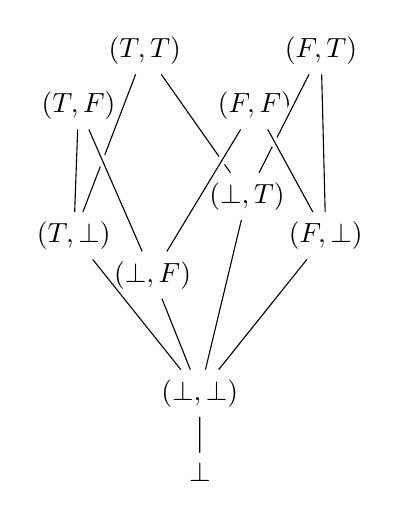
\begin{tikzpicture}

    \begin{scope}
        \myGlobalTransformation{0}{0};
        \node (bottom) at (0,0) {$\bot$};

        \myGlobalTransformation{0}{1};
        \node (botbot) at (0,0) {$(\bot,\bot)$};

        \myGlobalTransformation{0}{3};
        \node (trubot) at (-1,0) {$(\tru,\bot)$};
        \node (bottru) at (0,1)  {$(\bot,\tru)$};
        \node (falbot) at (1,0)  {$(\fal,\bot)$};
        \node (botfal) at (0,-1) {$(\bot,\fal)$};

        \myGlobalTransformation{0}{5};
        \node (trutru) at (-0.7, 0.7) {$(\tru,\tru)$};
        \node (faltru) at ( 0.7, 0.7) {$(\fal,\tru)$};
        \node (falfal) at ( 0.7,-0.7) {$(\fal,\fal)$};
        \node (trufal) at (-0.7,-0.7) {$(\tru,\fal)$};

        \draw (bottom) -- (botbot);

        \draw (botbot) -- (trubot);
        \draw (botbot) -- (bottru);
        \draw (botbot) -- (falbot);
        \draw (botbot) -- (botfal);

        \ddraw{trubot}{trutru};
        \ddraw{bottru}{trutru};
        \ddraw{falbot}{faltru};
        \ddraw{bottru}{faltru};
        \ddraw{trubot}{trufal};
        \ddraw{botfal}{trufal};
        \ddraw{botfal}{falfal};
        \ddraw{falbot}{falfal};

    \end{scope}

\end{tikzpicture}

%\end{document}
\caption{
    \texttt{(Bool,Bool)} partial order.
    \label{fig:boolboolcpo}
}
\end{center}
\end{wrapfigure} %\end{figure}
For tuples and other constructors that take other data types as
parameters, the ordering is:
\begin{equation*}
\hstup{x_0}{y_0} \sqsubseteq_{(a,b)} \hstup{x_1}{y_1} \text{\quad iff \quad}
x_0 \sqsubseteq_a x_1 \text{\w and \w} y_0 \sqsubseteq_b y_1
\end{equation*}

The Hasse Diagram for the \hs{(Bool,Bool)} values can be seen in
Figure \ref{fig:boolboolcpo}. Here \hs{True} is abbreviated for \hs{T}
and similarly for \hs{False}. It is not flat as the one for \hs{Bool};
it can be seen as three dimensional. On the lowest layer the only
value is $\bot$, on the next layer $\hstup{\bot}{\bot}$. Above that
the tuples with one $\bot$, and finally the total values at the
top.

\vspace{55pt}

\subsection{Monotonicity}
 An important property all safe Haskell functions have is that they are
monotone with respect to this ordering.

\paragraph{Definition} A function $f$ is \emph{monotone} iff

\begin{equation*}
\faa{x}{y} \quad x \sqsubseteq y \quad \Rightarrow \quad f(x) \sqsubseteq f(y).
\end{equation*}

This can be understood in many ways. One way to see it is if you have
two inputs to a function, one containing \emph{less} information that
the other, i.e. more bottoms, it is impossible to return \emph{more}
information from the input with less information.

\newpage

One simple example of a consequence of this is the impossibility to
make a function \hs{isBottom :: a -> Bool}, returning \hs{True} if the
argument is bottom, and \hs{False} otherwise:

\note{rewrite with code}
\begin{align*}
& \hs{isBottom} \w :: \hs{a} \rightarrow \hs{Bool} \\
& \hs{isBottom} \w \bot = \hs{True} \\
& \hs{isBottom} \w x \, = \hs{False}, \qquad x \neq \bot
\end{align*}

\noindent
Since $\bot \sqsubseteq x$ for any $x$, then by monotonicity we must
necessarily have
$$\hs{isBottom} \w \bot \sqsubseteq \hs{isBottom} \w x.$$
Take any non-bottom $x$, and this equation gives
$\hs{True} \sqsubseteq \hs{False}$, which is false. Hence
\hs{isBottom} is not monotone.

\subsection{Continuity}
Another domain theoretic property that Haskell functions have is that
they are continuous. This is a property that gives us insight in how
functions behave on infinite input.  To describe this, we need to
consider the partial order of a data type with infinite values. The
prime candidate \hs{data Nat = Zero | Succ Nat} is used and Hasse
Diagram can be seen in Figure \ref{fig:natcpo}.

\begin{figure}[h]
\centering
\usetikzlibrary{positioning,shadows,arrows}

\def\adots{\mathinner{\mkern2mu\raise\hbox{.}
\mkern2mu\raise4\hbox{.}\mkern1mu
\raise8\vbox{\kern7\hbox{.}}\mkern1mu}}


%\begin{tikzpicture}[scale=10]
%
%  \node (bottom)                          {$\bot$};
%  \node (zero)        [above=of bottom]   {$Zero$};
%  \node (suc bot)     [right=of zero]     {$Suc \, \bot$};
%  \node (suc zero)    [above=of suc bot]  {$Suc \, Zero$};
%  \node (suc suc bot) [right=of suc zero] {$Suc \, (Suc \, \bot)$};
%
%  \draw [-] (bottom) -- (zero);
%  \draw [-] (bottom) -- (suc bot);
%  \draw [-] (suc bot) -- (suc zero);
%  \draw [-] (suc bot) -- (suc suc bot);
%
%\end{tikzpicture}
%
\begin{tikzpicture}[grow'=up,sibling distance=2cm]
\node {$\bot$}
    child {
        node {$\hs{Zero}$}
    }
    child {
        node {$\hs{Succ} \, \bot$}
        child {
            node {$\hs{Succ} \, \hs{Zero}$}
        }
        child {
            node {$\hs{Succ} \, (\hs{Succ} \, \bot)$}
            child {
                node {$\hs{Succ} \, (\hs{Succ} \, \hs{Zero})$}
            }
            child {
              node {$ ^{ ^{\adots}}$}
              child [edge from parent/.style={draw=white}] { }
              child {
                node {$\hs{inf}$}
              }
            }
        }
    }

\end{tikzpicture}


\caption{
    The (complete) partial order for \texttt{Nat}, with \hs{inf = Succ inf.}
    \label{fig:natcpo}
}
\end{figure}

At the top we have the infinite value \hs{inf}, defined in Haskell as
\hs{inf = Succ inf}. Here \hs{inf} is the \emph{limit} of an
$\omega$-chain, i.e a chain with the same number of elements as
$\omega$, the natural numbers. The chain is:

\begin{equation*}
\bot \sqsubseteq
\hs{Succ} \, \bot \sqsubseteq
\hs{Succ} \, (\hs{Succ} \, \bot) \sqsubseteq
\hs{Succ} \, (\hs{Succ} \, (\hs{Succ} \, \bot)) \sqsubseteq
\cdots
\end{equation*}

This chain could succinctly be written $\langle \hs{Succ}^n \, \bot
\rangle_{n \in \omega}$.  Here $\hs{Succ}^n$ means $n$ applications of
the \hs{Succ} constructor. The limit is written $\lub{n \in
  \omega}(\hs{Succ}^n \, \bot)$ and is equal to \hs{inf}, where
$\lub{}$ is the least upper bound. All elements in the chain satisfy
the property of being less than or equal to the limit: $\hs{Succ}^n \,
\bot \sqsubseteq \hs{inf}$.

A partial order is a complete partial order iff there is a limit for
every $\omega$ chain. All data types in Haskell are complete partial
orders\footnote{Notice that the data type \hs{data StrictNat = Zero |
    Succ !StrictNat} is flat and therefore complete.}. Now we can
define continuity.

\paragraph{Definition} A function $f$ is \emph{continuous} iff it is
monotone and preserves the $\lub{ }$ of all $\omega$-chains: i.e.
assume any chain $\langle x_n \rangle_{n \in \omega}$, then:

\begin{equation*}
\lub{n \in \omega} \, (f \, x_n) \eq f \, (\lub{n \in \omega} \, x_n)
\end{equation*}

Just as with monotonicity, there are several ways to interpret
this. One way is to say that what a function does on a chain, it must
also do on the chain's limit, as with \hs{map} on increasingly longer
lists. Another is to say that a function cannot produce finite output by
inspecting infinite input: there is no function
\hs{isFinite :: [a] -> Bool} returning \hs{True} on finite lists and
\hs{False} on infinite lists. On the increasing chain
$$ \bot \sqsubseteq x_0 \hs{:} \bot \sqsubseteq x_0 \hs{:} x_1 \hs{:} \bot
\sqsubseteq \cdots$$
the function \hs{isFinite} returns \hs{True} (or $\bot$), but the
limit should return \hs{False}, so this is not a continuous function.

An interesting formulation of Church's Thesis in terms of continuity
is given by Plotkin \cite{domains}:

\begin{center}
\emph{A function is continuous iff it is physically feasible.}
\end{center}

This means that all computable functions are contiuous, and the other
way around. The conclusion for us is that all Haskell functions are
continuous.

\subsection{Unsafe Haskell}
In GHC, you can use \hs{unsafePerformIO} and \hs{catch} from
\hs{Control.Exception} and other tricks to unsafely catch errors
(bottoms). With this machinery it is possible to write a function
\hs{isBottom :: a -> Bool} to catch calls to \hs{undefined}, pattern
match failures, etcetera. In addition, some non-termination some can
also be catched in Haskell because of the \emph{blackhole} run time
object that replaces a \emph{thunk} that is being currently
evaluated. It does not and indeed cannot cover all non terminating
functions because of the undecidability of the Halting problem.

The domain theoretic results remain; one can see $\bot$ as another,
albeit inconveniently inspected, constructor to every data type. All
patterns are exhaustive: every function has an implicit match any
pattern to $\bot$.  Then we add a \emph{true} bottom to the domain
denotes the uncatchable bottoms; undeterminable non termination. With
this setting all Haskell functions are continuous with respect to the
\emph{true} bottoms. But for the rest of this thesis, we shall only
consider pure and safe Haskell functions.

\subsection{Monotonicity as Verification}

Continuity is a concept that is hard to express in first order logic:
it in not able to express countability. We can come close with an
axiomatization of set theory, but we leave that issue and focus on
monotonicity. A way to verify the translation is to add axioms to the
generated theory describing the $\sqsubseteq$ relation, and axioms
that asserts that each function is monotone. An automated theorem
prover could not easily show that it is a satisfiable theory since it
will normally only have infinite models. However, a long run without
any counter model could be seen as a witness for a successful
translation in this respect.


\section{Future Work}

Haskell is a big language, and translating it all in one go is a
daunting task. Therefore, some restrictions were settled to be able to
focus on proving rather than translating.  The goal was to add enough
of the Haskell language to enable to prove interesting properties, but
much of the widely available sugar in Haskell was omitted since it
does not add extra expressibility.

Some parts of Haskell that are not supported are list
comprehensions and do-notation can be added by its rewriting rules.
\hs{Type} definitions should be unrolled , so they could be used in
the signature for properties. Type classes is probably the most
interesting thing to add, and an approach would be to use dictionary
passing, and inline for concrete types. However, more type information
would be needed but it is possible that much of it could be extracted
from example GHC. Since type classes are not not translated,
higher-kinded type variables are neither.

Another interesting but omitted feature are the built-in types like
\hs{Int}, \hs{Integer}, \hs{Double}, \hs{Char}, etc. For \hs{Integer}
appropriate axioms could be added that hold for $\mathbb{Z}$, the
canonical infinite discretely ordered commutative ring. For the other
data types it is as simple because of different bit sizes and overflow
and precision errors.

Syntactic features for controlling lazy and strict evaluation like
irrefutable patterns, \hs{seq} and bang patterns, and richer pattern
matching in form of pattern bindings are discussed below, but it
should be noted that it is already possible to prove a lot of
interesting Haskell properties, it is far from able to prove things
about bigger Haskell projects which usually use a richer part of the
language.

\subsection{Irrefutable Patterns and Pattern Bindings}

Irrefutable patterns can be defined in terms of strict projections,
like those that already exist (\hs{fst}, \hs{snd}, \hs{head},
\hs{fromJust}, and so on.) Each irrefutable pattern is translated to a
constant, and when you use the variables in the pattern, you translate
it to appropriate use of strict projections. One example is the
translation of the \hs{uncurry} function:

\begin{code}[mathescape]
uncurry f ~(x,y) = f x y        $\Leftrightarrow$      uncurry f t = f (fst t) (snd t)
\end{code}

\noindent
The irrefutable pattern \verb:~(x,y): is replaced with the new constant
\hs{t}, and in the body of the function, \hs{x} is replaced with the
strict projection \hs{fst t}, and similarly for \hs{y}.

Top level patterns, more specifically called pattern bindings, can
also be written in terms of such strict projections. The whole pattern
is replaced with a constant, and when the variables from the pattern
are used, you again replace it with strict projections. This is how it
could look for a simple \hs{fromJust . lookup} implementation:

\begin{code}[mathescape]
unsafeLookup x xs = v           $\Leftrightarrow$      unsafeLookup x xs = fromJust t
  where Just v = lookup x xs            where t = lookup x xs
\end{code}

The strict projections would not rely on the user having \hs{fst} or
\hs{fromJust} in scope, they can automatically be generated by
inspection of the data type definition.

\subsection{Bang Patterns and seq}

The encoding for bang patterns and \hs{seq} is also straightforward,
say you want to define seq with bang patterns, you would have

\begin{code}
seq :: a -> b -> b
seq !x y = y
\end{code}

The axioms needs to ensure that if \hs{x} evaluates to $\bot$, then
\hs{seq x} also evaluates to $\bot$. The two axioms for this functions are:
\begin{align*}
\rom{1} \qquad & \fa{y}    seq(\bot,y) \eq \bot \\
\rom{2} \qquad & \faa{x}{y} x \neq \bot \rightarrow seq(x,y) \eq y
\end{align*}

Either you implement bang patterns in this fashion, or you do the same
translation as GHC for bang patterns: for each strict variable, you
add a \hs{seq} for that variable for the expression of that pattern,
and you simply add the axioms for \hs{seq} to the theory if the
program uses it or bang patterns. This also works for data types with
strictness fields.

\subsection{Pattern Guards}

Patterns guards is a GHC specific extension to Haskell, allowing
arbitrary pattern matching on an expression in a guard. An example is
this elaboration of the \hs{lookup} function from the \hs{Prelude},
which applies a function to the element, if found:

\begin{code}
transformLookup :: Eq k => k -> [(k,v)] -> (k -> v -> b) -> Maybe b
transformLookup k xs f | Just v <- lookup k xs = Just (f k v)
                       | otherwise             = Nothing
\end{code}

\noindent
If the lookup returns \hs{Just}, you already have the value \hs{v}
bound and can use it in the expression for this pattern. This is not
at all unlike the normal guards, they are a special case of pattern
guards: the guard \hs{f x | p x} is expressed as
\hs{f x | True <- p x}. The translation of guards currently checks if
\hs{p x} is \hs{True}, and then ``picks'' this branch, or $\bot$ and
then ``returns'' $\bot$. You could just as well do this for other
constructors, you just need to add bottoms in the guard branches just
as is currently done for ordinary patterns.

